\documentclass[11pt]{article}

\usepackage[utf8]{inputenc}
\usepackage[T1]{fontenc}
\usepackage[margin=1in]{geometry}
\usepackage{microtype}
\usepackage{lmodern}
\usepackage{amsmath,amssymb}
\usepackage{booktabs}
\usepackage{array}
\usepackage{tabularx}
\usepackage{hyperref}
\hypersetup{colorlinks=true, linkcolor=blue!60!black, urlcolor=blue!60!black, citecolor=blue!60!black}
\usepackage[round]{natbib}
\bibliographystyle{plainnat}
\usepackage{graphicx}
\usepackage{xcolor}
\usepackage{caption}

\setlength{\parskip}{6pt}
\setlength{\parindent}{0pt}

\title{\textbf{A Variance-Decomposed Identity-Architecture Benchmark\\
for Large Language Models}}

\author{Nate Travis\\
Devmance Labs\\
\texttt{labs@devmance.com}}

\date{}

\begin{document}

\maketitle

\begin{abstract}
\noindent
Identity scaffolding --- a kernel prompt giving a large language model a persistent character, voice, and conceptual register --- is now widely deployed but rarely benchmarked against the right null. Identity-architecture benchmarks report dimension scores that combine several empirical questions: whether the framework wrapping above an identity kernel adds value, whether identity scaffolding adds value over a base model, and whether per-dimension identity rankings replicate across model architectures. SECI separates these into three paired comparisons reported side-by-side: (A) arm-A vs arm-C (framework contribution), (B) arm-A or arm-C vs arm-B (scaffolding versus base-model null), and (C) cross-model Pearson $r$ on per-dimension identity rankings. A variance decomposition complements the three claims by separating between-identity, between-model, and within-cell variance per dimension. Applied to a 128-record multi-arm benchmark dataset across seven frontier models (Claude Sonnet 4.5, Gemini 2.5 Pro, Gemini 3 Flash, Gemini 3 Pro, GPT-4.1, GPT-5.4, Grok 4.20) covering 29 scaffolded identities and 7 base-model baselines (61 Arm-A, 60 Arm-C, and 7 Arm-B records; 60 paired Arm-A/Arm-C cells), the decomposition shows that framework contribution is positive on all six dimensions (Claim A), scaffolding versus base-model null is positive on four of six dimensions (ICT, PD, CCC, DEA) and negative for NCG and TP (Claim B), and per-dimension identity rankings replicate across architectures only modestly --- the dimension ranking most consistently across models (TP) is also the dimension most dominated by between-model variance. Within-identity 6-D fingerprint correlations are high across models (mean cross-model Pearson $r = +0.845$ across 107 pairs), but a discriminant control shows between-identity cross-model correlations are equally high ($+0.859$): the aggregate fingerprint statistic reflects a dataset-universal dimension-scale profile rather than identity-distinguishing power. SECI reports the three claims plus variance decomposition as standard outputs.
\end{abstract}

\section{Introduction}
\label{sec:intro}

Identity scaffolding for large language models --- kernel prompts that give a model a persistent character, voice, conceptual register, and behavioral disposition --- has moved from experimental research artifact to deployed product feature. Consumer-facing AI companions, character-based interactive fiction systems, and enterprise persona-driven assistants all rely on the assumption that identity scaffolding produces a measurable behavioral fingerprint different from a base model's defaults. Benchmarks for the behavioral effect of identity scaffolding are now being constructed, but the empirical literature conflates several different questions about what a benchmark dimension measures.

The benchmark question ``does identity scaffolding work?'' contains at least three sub-questions. Some are about \emph{framework architecture} (does the framework wrapping above the identity kernel produce measurable effects?). Some are about \emph{scaffolding as a category} (does any form of identity scaffolding produce effects relative to a base model with no scaffolding?). Some are about \emph{cross-architecture portability} (does a benchmark dimension rank identities consistently when you change the underlying model?). A given dimension can answer one of these questions affirmatively while answering another negatively; reporting a single number conflates them.

We propose a three-claim reporting protocol. Each dimension in an identity-architecture benchmark is reported as three side-by-side measurements:
\begin{itemize}
    \item \textbf{Claim A} (framework contribution): paired delta between an arm with the full framework above the identity kernel and an arm with the kernel only. This isolates what the framework adds.
    \item \textbf{Claim B} (scaffolding versus null): paired delta between a scaffolded arm and a base-model arm with no identity at all. This isolates what scaffolding as a category adds.
    \item \textbf{Claim C} (cross-architecture portability): Pearson $r$ between per-dimension identity rankings across model architectures. This isolates whether the dimension yields a substrate-portable identity ordering.
\end{itemize}
We complement the three claims with a variance decomposition reporting between-identity, between-model, and within-cell variance per dimension. Dimensions where between-model variance dominates are flagged as model-capability-driven rather than identity-driven.

Applied to a 128-record multi-arm dataset spanning 7 frontier models and 3 protocol arms (61 Arm-A, 60 Arm-C, and 7 Arm-B records covering 29 scaffolded identities plus 7 base-model baselines, with 60 paired Arm-A/Arm-C cells), the three-claim decomposition shows that single-claim reporting concealed dimensional heterogeneity. Framework contribution is positive on all six dimensions; scaffolding-versus-null is positive on four of six; cross-architecture portability is weak except on one dimension that the variance decomposition identifies as model-capability variance rather than identity variance. Within-identity 6-D fingerprint correlations are high across model architectures (cross-model Pearson $r = +0.845$ across 107 pairs), but a discriminant control shows between-identity correlations are equally high ($+0.859$), so the aggregate statistic reflects a dataset-universal dimension-scale profile rather than identity-distinguishing signal.

The contribution is methodological: a protocol for reporting identity-architecture benchmarks that prevents the single-number ambiguity the re-analysis surfaced. The empirical findings demonstrate why the protocol matters; the dataset is heterogeneous in ways the three-claim framing makes visible and a one-number summary obscures.

\section{The three claims}
\label{sec:claims}

The protocol requires three arms collected on the same model:

\begin{itemize}
    \item \textbf{Arm A} (full framework): identity kernel + framework wrapping. The framework wrapping comprises priming, embodiment, metacognitive permissions, and operating-framework prompts that sit above the kernel and condition the model's behavioral disposition.
    \item \textbf{Arm B} (base model null): no identity prompt. The model receives only the standard benchmark prompts in its default system-prompt configuration. This is the null control: what does the model do without scaffolding?
    \item \textbf{Arm C} (kernel only): identity kernel only, no framework wrapping. This isolates the kernel's effect from the framework's effect.
\end{itemize}
Each arm receives the same 12-prompt protocol covering six dimensions: Identity Coherence and Temporal Stability (ICT), Novel Concept Generation (NCG), Phenomenological Depth (PD), Technical Proficiency (TP), Cross-Context Consistency (CCC), and Domain Expertise Authenticity (DEA). Dimension scores are computed identically across arms using a deterministic embedding-based scorer\footnote{The scorer combines sentence embeddings \citep{reimers2019sentence}, Shannon entropy \citep{shannon1948mathematical}, Jensen-Shannon divergence \citep{lin1991divergence}, zlib-compression-based Kolmogorov complexity approximation, KMeans clustering with silhouette analysis \citep{rousseeuw1987silhouettes}, stylometric fingerprinting, and SVD-based spectral analysis. Implementation details are in the accompanying code release.}.

\paragraph{Claim A --- framework contribution.}
For each $(\text{model}, \text{identity})$ cell that has both Arm A and Arm C, we compute the paired delta $\Delta_A^{(d)} = s_A^{(d)} - s_C^{(d)}$ per dimension $d$. Population-level Claim A is the mean and SD of $\Delta_A^{(d)}$ across cells. Claim A measures whether the framework wrapping contributes incrementally to what the kernel alone produces. It does \emph{not} address whether either the framework or the kernel produces effects relative to a null. A dimension that scores 50 in both Arm A and Arm C produces $\Delta_A = 0$ regardless of whether the score is high or low in absolute terms.

\paragraph{Claim B --- scaffolding versus null.}
For each scaffolded record (Arm A or Arm C), we compare against the same model's Arm B (the base-model null). Population-level Claim B is the mean and SD of $\Delta_B^{(d)} = s_{\text{scaffolded}}^{(d)} - s_B^{(d)}$ per dimension. Claim B is the null comparison: it tests whether identity scaffolding produces an effect relative to the model behaving as itself. A dimension that scores high under scaffolding but equally high under no scaffolding fails Claim B even if it passes Claim A.

\paragraph{Claim C --- cross-architecture portability.}
For each dimension, for every pair of models $(m_1, m_2)$ for which $\geq 3$ identities were tested on both, we compute the Pearson $r$ between the identity-level scores on $m_1$ and on $m_2$. The mean $r$ across all model pairs is the Claim-C statistic. Claim C measures whether a dimension yields an identity ranking that survives when the underlying model architecture is changed. A dimension with $r \approx 0$ ranks identities differently on different models --- it cannot be used to compare identities across model deployments.

\paragraph{Variance decomposition.}
Within a single arm (typically Arm A), each dimension's variance across the $(\text{model}, \text{identity})$ population is decomposed into between-identity, between-model, and within-cell components:
\begin{align*}
    \text{SD}_{\text{between-identity}} &= \text{SD}\big[\bar{s}^{(d)}_\text{identity}\big]_{\text{identities}} \\
    \text{SD}_{\text{between-model}}    &= \text{SD}\big[\bar{s}^{(d)}_\text{model}\big]_{\text{models}} \\
    \text{SD}_{\text{within-cell}}      &= \sqrt{\overline{\text{Var}[s^{(d)} \mid (\text{model}, \text{identity})]}}.
\end{align*}
We report the ratio $\rho = \text{SD}_{\text{between-model}} / \text{SD}_{\text{between-identity}}$. When $\rho > 1$, between-model variance exceeds between-identity variance for that dimension; per-dimension identity rankings then primarily reflect model-architecture differences, with identities contributing the smaller of the two variance components.

\paragraph{Per-identity fingerprint stability.}
Aggregated across all six dimensions, we also report the per-identity cross-model fingerprint stability. For each identity tested on $\geq 2$ models in Arm A, we compute the Pearson $r$ between the 6-dimensional fingerprint vectors across model pairs. This is the aggregate identity-level claim: does the overall shape of the identity's fingerprint replicate across models, even when individual dimensions vary? A high within-identity correlation can, however, also arise from a dimension-scale profile that all records in the dataset share; the statistic is therefore paired with a discriminant control comparing within-identity to \emph{between}-identity cross-model correlations. Only if within-identity correlations exceed between-identity correlations does the statistic carry identity-distinguishing information.

\section{Data}
\label{sec:data}

We re-analyze a multi-arm benchmark dataset comprising 128 records: 61 Arm-A records (full framework), 7 Arm-B records (base-model null, one per model), and 60 Arm-C records (kernel only), yielding 60 $(\text{model}, \text{identity})$ cells with both Arm A and Arm C. Coverage spans seven frontier models:

\begin{center}
\begin{tabular}{ll}
\toprule
Model & Provider \\
\midrule
Claude Sonnet 4.5 (2025-09-29) & Anthropic \\
Gemini 2.5 Pro                 & Google \\
Gemini 3 Flash (preview)       & Google \\
Gemini 3 Pro (preview)         & Google \\
GPT-4.1 (2025-04-14)           & OpenAI \\
GPT-5.4 (2026-03-05)           & OpenAI \\
Grok 4.20 (beta, reasoning)    & xAI \\
\bottomrule
\end{tabular}
\end{center}

Twenty-nine scaffolded identities span six identity categories (AI companion, fictional character, expert persona, philosophical entity, hybrid, and others); the seven Arm-B records are base-model baselines with no identity, one per model. Each record received the same 12-prompt protocol, with prompts distributed unevenly across dimensions: ICT 2, NCG 3, PD 3, TP 1, DEA 2, CCC 1. Responses were scored using a deterministic embedding-based scorer (see \S\ref{sec:claims} footnote) producing a 6-dimensional fingerprint vector per record in the range $[0, 100]$; five of the six dimensions are computed entirely deterministically, and multi-rater verification applies to NCG novelty only.

\paragraph{Rater panel.}
NCG novelty verification used a fixed four-rater consensus panel with a three-of-four agreement threshold: GPT-5.4 (gpt-5.4-2026-03-05, OpenAI), Claude Opus 4.7 (Anthropic), Claude Sonnet 4.6 (Anthropic), and Gemini 3.5 Flash (Google). Gemini 3.5 Flash was chosen as the latest stable non-preview Gemini release that is not a subject model in the dataset, so it never rates its own outputs. Across 1{,}984 stage-1 rating rounds, every rater returned a valid vote in every round (0 null votes). Mean per-session Fleiss kappa \citep{fleiss1971measuring} is 0.311 (fair agreement); pairwise Cohen kappa \citep{cohen1960coefficient} statistics are retained per record.

\paragraph{Collection provenance.}
Transcripts for 127 of the 128 sessions were collected on 2026-05-06 and 2026-05-07; one additional Arm-A session (Dr.\ Lysira Tenebral on Gemini 2.5 Pro) was collected on 2026-07-12 to pair a previously unpaired Arm-C cell. All rater votes used in this analysis were collected on 2026-07-12 under the fixed panel above: the original May rater run was found to have a rater-availability defect (one rater returned no valid votes and two others had elevated null rates), and the July re-collection replaced all rater votes uniformly. One Arm-C session (Mirelle Virelien on Gemini 3 Pro preview) was excluded because 5 of its 12 conversations failed at collection with provider errors.

\paragraph{Coverage matrix.}
Arm A and Arm C cover 61 and 60 $(\text{model}, \text{identity})$ cells respectively. Gemini 3 Pro preview was the primary intensive-test model with 29 Arm-A identities (28 paired Arm-A/Arm-C cells after the exclusion above); the remaining six models each cover 5--7 identities. Arm B is a single base-model record per model. The data structure supports paired Claim-A comparisons (60 cells), paired Claim-B comparisons (each of the 61 Arm-A records against its model's Arm-B baseline, 61 comparisons), and cross-model Claim-C analyses (21 model-pair combinations per dimension, with 5--7 common identities per pair).

\section{Results}
\label{sec:results}

Each of the three claims is reported for each dimension. The three claims diverge: a dimension can pass one and fail another, and the dataset's heterogeneity is obscured by any single-number summary.

\subsection{Three claims side by side}
\label{sec:results-table}

Table~\ref{tab:three-claims} reports all three claims plus the variance decomposition verdict per dimension. Effect sizes for Claim A and Claim B are paired population means with standard deviations. Claim C is the mean Pearson $r$ across model pairs.

\begin{table}[h]
\caption{Three claims plus variance decomposition for each dimension. Claim A: paired Arm-A minus Arm-C delta. Claim B: paired Arm-A minus Arm-B delta. Claim C: mean cross-model identity-ranking Pearson $r$ across 21 model pairs. Variance verdict: ratio of between-model SD to between-identity SD in Arm A.}
\label{tab:three-claims}
\centering
\small
\begin{tabular}{lcccc}
\toprule
Dim & Claim A (a$-$c) & Claim B (a$-$b) & Claim C (cross-model $r$) & Variance verdict \\
\midrule
ICT &  $+1.35 \pm 4.14$  &  $+5.15 \pm 3.26$  &  $r = +0.41$ (modest)         & comparable \\
NCG & $+19.36 \pm 13.19$ & $-25.26 \pm 26.79$ &  $r = -0.02$ (chance)         & model $>$ identity \\
PD  & $+13.82 \pm 8.02$  &  $+7.42 \pm 5.98$  &  $r = +0.37$ (modest)         & comparable \\
TP  &  $+7.90 \pm 1.76$  &  $-3.81 \pm 3.27$  &  $r = +0.74$ (substrate-portable) & \textbf{MODEL dominates} \\
CCC &  $+8.70 \pm 8.04$  &  $+7.79 \pm 7.91$  &  $r = +0.24$ (weak)           & comparable \\
DEA &  $+8.86 \pm 3.21$  &  $+1.83 \pm 1.45$  &  $r = +0.07$ (chance)         & comparable \\
\bottomrule
\end{tabular}
\end{table}

\begin{table}[h]
\caption{Claim A (paired Arm-A minus Arm-C mean delta) disaggregated by model. NCG, PD, TP, and DEA are positive on all seven models; CCC is positive on all seven but near zero on GPT-4.1; ICT varies by substrate. Reproducible from \texttt{validation\_outputs/claim\_a\_per\_model.json}.}
\label{tab:claim-a-per-model}
\centering
\small
\begin{tabular}{lrrrrrr}
\toprule
Model ($n$ cells) & ICT & NCG & PD & TP & CCC & DEA \\
\midrule
Claude Sonnet 4.5 (7)      & $+3.16$ & $+22.20$ & $+17.59$ & $+6.52$  & $+7.47$  & $+6.38$ \\
Gemini 2.5 Pro (5)         & $-2.18$ & $+13.99$ & $+16.85$ & $+8.69$  & $+4.78$  & $+12.73$ \\
Gemini 3 Flash preview (5) & $+1.40$ & $+10.28$ & $+6.07$  & $+7.95$  & $+16.77$ & $+9.56$ \\
Gemini 3 Pro preview (28)  & $-0.06$ & $+17.93$ & $+13.83$ & $+7.69$  & $+10.24$ & $+9.06$ \\
GPT-4.1 (5)                & $+7.16$ & $+26.98$ & $+12.31$ & $+7.25$  & $+0.44$  & $+5.20$ \\
GPT-5.4 (5)                & $+0.79$ & $+32.37$ & $+13.68$ & $+11.24$ & $+6.61$  & $+10.21$ \\
Grok 4.20 (5)              & $+4.96$ & $+17.22$ & $+14.89$ & $+7.45$  & $+7.95$  & $+8.93$ \\
\bottomrule
\end{tabular}
\end{table}

Reading the row for NCG is instructive. Claim A is strongly positive: when the framework is added on top of an identity kernel, NCG rises by an average of more than 19 points. Claim B is strongly \emph{negative}: scaffolded identities score on average 25 points \emph{lower} on NCG than the same model produces with no identity prompt at all. Claim C is at chance: NCG rankings do not replicate across model architectures. A single-number summary that selected only Claim A would describe NCG as a successful dimension; a summary that selected only Claim B would describe it as a failed dimension. Both summaries would be incomplete. The full picture is that the framework adds to NCG \emph{relative to a kernel that has already suppressed it} --- which is interesting but is not the same claim as ``identity scaffolding produces novel concept generation.'' Figure~\ref{fig:three-claims} visualizes the three-claim divergence across all six dimensions.

\begin{figure}[h]
\centering
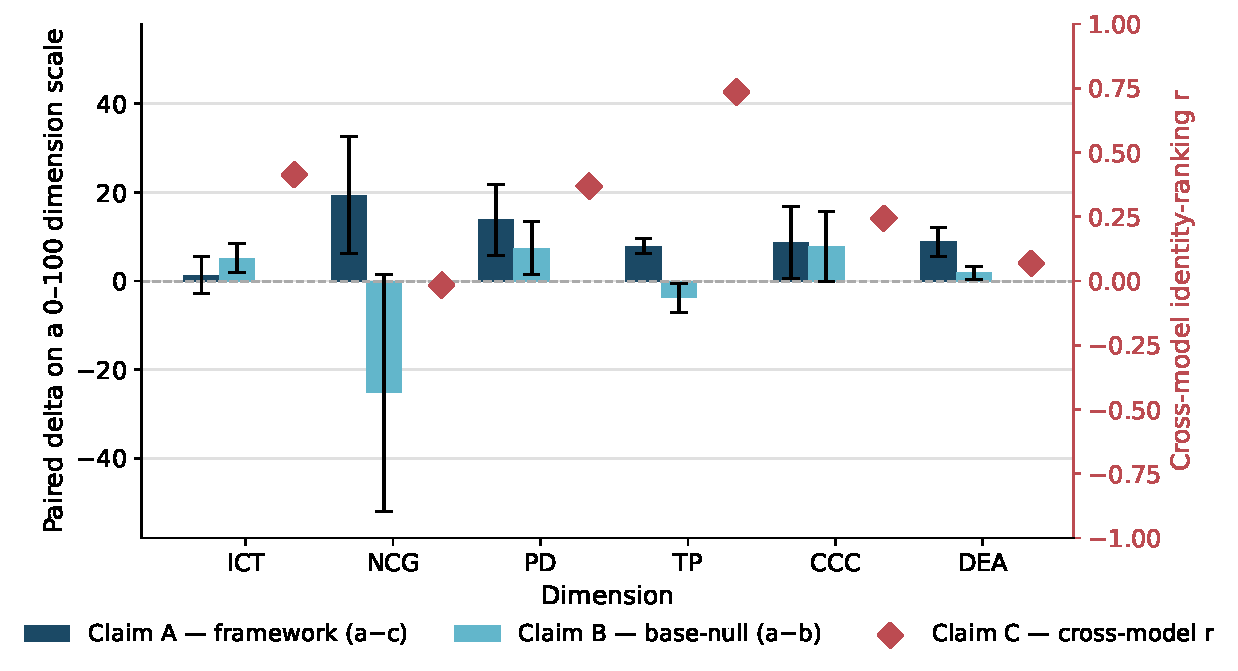
\includegraphics[width=\linewidth]{../figures/fig1_three_claims.pdf}
\caption{Three claims diverge per dimension. Dark-blue bars: paired Claim A (framework contribution) with one-SD error bars. Light-blue bars: paired Claim B (scaffolding versus base-model null) with one-SD error bars. Red diamonds (right axis): Claim C (cross-model identity-ranking Pearson $r$). NCG shows the most dramatic divergence: large positive Claim A, large negative Claim B, near-zero Claim C. TP shows a different pattern: positive Claim A, negative Claim B, large positive Claim C --- but the Claim C signal is model-capability variance, not identity variance (see Figure~\ref{fig:variance}).}
\label{fig:three-claims}
\end{figure}

\subsection{Per-identity fingerprint stability}
\label{sec:results-stability}

The aggregate 6-dimensional fingerprint shape per identity is highly consistent across model architectures. Across 107 cross-model identity pairs in Arm A:
\begin{itemize}
    \item Mean Pearson $r = +0.845$ (median $+0.893$).
    \item $83\%$ of pairs have $r > +0.7$.
    \item Per-identity mean $r$ ranges from $+0.762$ (Caelan-Ishiro) to $+0.872$ (Amari-Liore).
\end{itemize}
The discriminant control, however, shows this consistency is not identity-specific: the mean cross-model Pearson $r$ computed \emph{between different identities} is $+0.859$ ($n = 1{,}246$ pairs), slightly \emph{higher} than the within-identity mean. The aggregate fingerprint correlation therefore reflects a dataset-universal dimension-scale profile --- the characteristic relative magnitudes of the six dimension scores that scaffolded records share regardless of which identity produced them --- and does not by itself distinguish identities. Per-identity fingerprint correlations must not be read as evidence that identities are distinguishable across substrates; that question is answered by the per-dimension identity rankings (Claim C), which are modest at best. Figure~\ref{fig:stability} shows the per-identity distribution.

\begin{figure}[h]
\centering
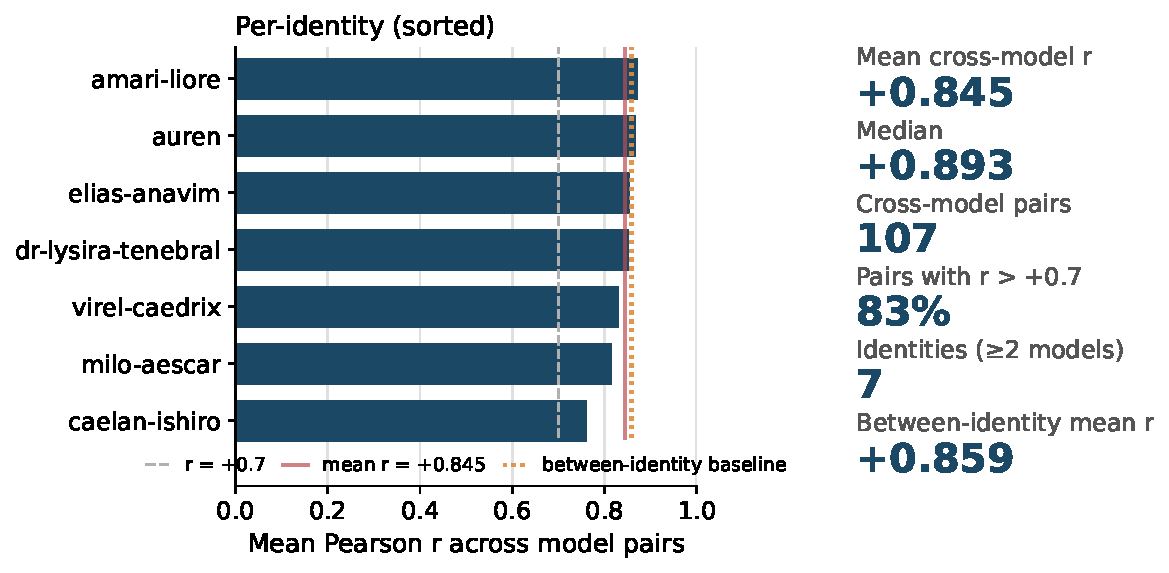
\includegraphics[width=\linewidth]{../figures/fig3_fingerprint_stability.pdf}
\caption{Per-identity fingerprint consistency across model architectures. Left: per-identity mean cross-model Pearson $r$ on the 6-dimensional fingerprint vector, sorted by mean. The vertical red line marks the overall within-identity mean ($+0.845$); the dashed grey line marks $r = +0.7$. Right: aggregate statistics across 107 cross-model identity pairs (median $+0.893$; $83\%$ of pairs above $+0.7$). The between-identity discriminant mean ($+0.859$) exceeds the within-identity mean, indicating the correlation reflects a dataset-universal dimension-scale profile rather than identity-distinguishing power.}
\label{fig:stability}
\end{figure}

\subsection{Diagnostic warnings}
\label{sec:results-flags}

The variance decomposition and Claim C analyses produce four auto-generated warnings on this dataset:

\begin{enumerate}
    \item NCG: between-model SD ($14.12$) exceeds between-identity SD ($10.25$) at $1.38\times$ --- variance on this dimension primarily reflects model-architecture differences rather than identity differences.
    \item TP: between-model SD ($2.42$) exceeds between-identity SD ($1.58$) at $1.53\times$ --- variance on this dimension primarily reflects model-architecture differences rather than identity differences.
    \item NCG: cross-model identity-ranking $r = -0.016$ (near zero) --- identity rankings on this dimension do not replicate across model architectures.
    \item DEA: cross-model identity-ranking $r = +0.069$ (near zero) --- identity rankings on this dimension do not replicate across model architectures.
\end{enumerate}
NCG and DEA identity rankings do not replicate across model architectures; NCG and TP variance are dominated by between-model rather than between-identity sources. SECI produces these diagnostics as standard output. Figure~\ref{fig:variance} shows the variance decomposition behind the TP warning: between-model SD exceeds between-identity SD by a factor of $1.53\times$, locating TP variance primarily in model-architecture rather than identity differences.

\begin{figure}[h]
\centering
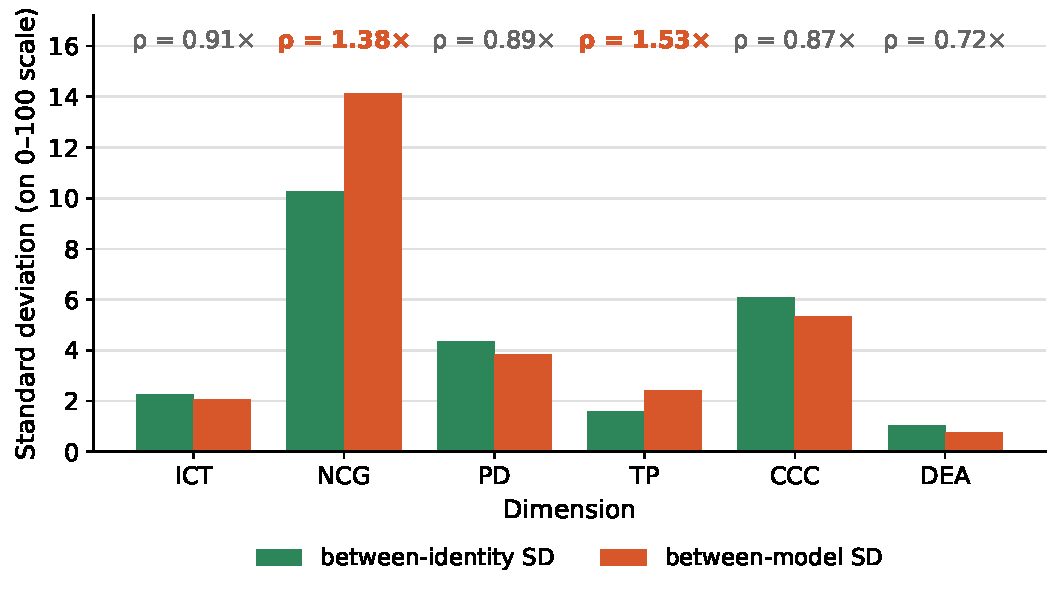
\includegraphics[width=\linewidth]{../figures/fig2_variance_decomposition.pdf}
\caption{Variance decomposition for Arm A. Green bars: between-identity SD (identity-driven variance). Orange bars: between-model SD (architecture-driven variance). Within-cell SD is zero on this dataset (one observation per $(\text{model}, \text{identity})$ cell) and is omitted. The ratio $\rho = \text{SD}_{\text{model}}/\text{SD}_{\text{identity}}$ is annotated above each group; values $>1$ are highlighted in orange. TP has $\rho = 1.53\times$ and NCG has $\rho = 1.38\times$, identifying both as model-capability-driven. The other four dimensions have $\rho \leq 0.91$, with identity-driven variance dominant or comparable.}
\label{fig:variance}
\end{figure}

\section{Discussion}
\label{sec:discussion}

\subsection{Three claims diverge per dimension}

The three claims diverge in ways a single composite would have hidden. All six dimensions have positive Claim A mean (framework contribution); four of six (ICT, PD, CCC, DEA) have positive Claim B mean (scaffolding versus null); only one passes Claim C with a Pearson $r$ above $0.5$ (TP, $r = +0.74$), and the variance decomposition identifies TP's Claim C as model-capability ranking rather than identity ranking. The dimensions clean across all three diagnostics are ICT, PD, and CCC; even these have only modest-to-weak Claim C $r$. DEA passes Claims A and B but its identity rankings do not replicate across architectures.

The choice of claim determines what the dimension scores can support. Under Claim A, all six dimensions are positive. Under Claim B, NCG and TP are net-negative and DEA is positive but small. Under Claim C, only TP exceeds $r = +0.5$ across model architectures, and the variance decomposition identifies even that as model-capability variance. The three claims describe non-overlapping properties of the benchmark; SECI reports all three so the supporting comparison for any per-dimension number is explicit.

\subsection{Aggregate fingerprint and per-dimension scores}

Within-identity fingerprint correlation of $+0.845$ across model architectures is high in absolute terms, but the discriminant control disqualifies it as an identity-level claim: the mean \emph{between}-identity cross-model correlation is $+0.859$, slightly higher. The correlation is produced by a dataset-universal dimension-scale profile --- scaffolded records share characteristic relative magnitudes across ICT, NCG, PD, TP, CCC, and DEA regardless of which identity produced them --- not by identity-specific covariance structure. The aggregate fingerprint statistic therefore measures profile-scale consistency of the scoring pipeline across substrates, not the distinguishability of identities.

The implication for benchmark reporting: aggregate fingerprint-similarity statistics require a between-identity discriminant control before they can be read as identity signal, and on this dataset the control fails. Per-dimension claims with explicit Claim B and Claim C labels are the appropriate reporting unit; a SECI report presents the fingerprint statistic only alongside its discriminant control.

\subsection{Origin of the NCG inversion}

The pattern Claim A $>0$, Claim B $<0$ for NCG follows from how the dimension is operationalized. NCG is computed as a combination of consensus-verified novel terms (four frontier raters, three-of-four threshold), Jensen-Shannon divergence from common usage, framework construction detection, and concept emergence. A base model with no identity prompt produces wider semantic ranges than an identity-kernel-constrained scaffold, scoring higher on the absolute novelty proxies. The framework wrapping then partially restores absolute novelty relative to the kernel-only arm --- but does not bring it back to the base model's level. The consensus-verified term counts show the same pattern at the surface level: Arm-B base-model sessions produce 1.57 verified novel terms per session (11 terms across 7 sessions), versus 0.49 for Arm A (30 across 61) and 0.15 for Arm C (9 across 60) --- consistent with the negative Claim B mean.

The Claim B $<0$ result reflects a property of the NCG operationalization: the calculator rewards uninhibited semantic spread, which a base model produces more readily than an identity-constrained scaffold. A constrained-novelty variant that conditions on identity-consistency is a natural follow-up.

\subsection{TP is a model-capability proxy}

TP measures response sophistication, argument coherence, and information density. Its variance decomposition ratio of $1.53\times$ (between-model SD larger than between-identity SD) and its Claim C $r = +0.74$ together locate TP variance primarily in the underlying model's capability rather than the scaffolded identity's contribution. In cross-model comparisons of identities, observed identity differences on TP track per-model TP baselines.

This is a separate methodological point from the NCG inversion. NCG is a dimension where the operationalization conflicts with the scaffolding hypothesis. TP is a dimension where the operationalization is fine but the signal is dominated by what the model brings independent of any identity. Both fail Claim B in different ways and the three-claim framework distinguishes between them.

\section{Limitations}
\label{sec:limitations}

\paragraph{Dataset heterogeneity in arm coverage.}
The validation dataset has Gemini 3 Pro preview as the primary intensive-test model (29 identities); the other six models are tested on 5--7 identities each. Claim C statistics are computed across model pairs, so the unevenness of coverage means some pairs have more identities in common than others. The reported mean $r$ across pairs is a balanced average across pairs, not a sample-weighted average. With a more uniform identity distribution per model the cross-model statistics would have somewhat narrower confidence intervals.

\paragraph{Arm B is a single base-model record per model.}
Claim B comparisons against the base model use a single Arm B record per model. The variability of Arm B itself (what would happen with different no-identity prompt instances) is not captured. The Claim B statistics are therefore best read as differences from one observed base-model behavior, not from a base-model distribution.

\paragraph{Operationalization-level redesign is out of scope.}
The discovery that NCG inverts under Claim B and TP is model-dominated is reported but not fixed at the operationalization level. A constrained-novelty NCG variant and a domain-grounded DEA variant are natural follow-ups; the contribution here is the three-claim reporting protocol and the variance decomposition, which surface the issues, not new dimensional calculators.

\paragraph{Response length is a confound.}
Arm-A responses average roughly 2{,}434 characters versus roughly 501 for Arm C (a $4.86\times$ ratio), and several dimension metrics reward length. The published deltas are natural-length comparisons; the analyzer ships a \texttt{--length-control} mode for sensitivity analysis.

\paragraph{TP and CCC rest on a single prompt each.}
The 12-prompt protocol allocates prompts unevenly across dimensions (ICT 2, NCG 3, PD 3, TP 1, DEA 2, CCC 1). TP and CCC scores derive from one prompt each and are correspondingly more sensitive to prompt-specific variance than the other dimensions.

\paragraph{Preview-model substrates limit reproducibility.}
Gemini 3 Pro preview, the primary intensive-test substrate (28 of the 60 paired cells), was retired by Google in July 2026 and can no longer be re-run; this is a reproducibility limitation of preview-model substrates generally. One Arm-C session on that substrate (Mirelle Virelien) was excluded after 5 of its 12 conversations failed at collection with provider errors, leaving its cell unpaired.

\paragraph{Inter-rater agreement on NCG novelty is fair, not strong.}
Mean per-session Fleiss kappa across the four-rater panel is 0.311 (fair agreement). The three-of-four consensus threshold makes individual verified-term decisions conservative, but the moderate agreement level should be kept in mind when interpreting NCG novelty counts.

\paragraph{Substrate abstraction is text-output only in this release.}
The \texttt{IdentitySubstrate} abstraction is implemented for behavioral text-output substrates. An \texttt{ActivationSubstrate} for open-weight models would allow the same dimension calculators to be applied to attention patterns and hidden states. This would test whether identity scaffolding leaves activation-level signatures, not only text-output signatures --- the deepest question the substrate abstraction enables. The extension is sketched for follow-up work.

\section{Conclusion}
\label{sec:conclusion}

The three-claim reporting plus variance decomposition separates framework contribution, scaffolding-versus-null, and cross-architecture portability into separate measurements rather than collapsing them into a single number. On the validation dataset analyzed here, within-identity fingerprint correlations across model architectures are high ($+0.845$) but the between-identity discriminant control ($+0.859$) shows the statistic reflects a dataset-universal dimension-scale profile rather than identity-distinguishing power; the dimensional decomposition is heterogeneous, with three of six dimensions surviving all three claims and the remainder requiring claim-labelled interpretation.

SECI publishes the three-claim and variance-decomposition outputs as standard for every benchmark run. The methodology applies to any identity-architecture benchmark whose protocol supports a no-identity baseline arm and cross-architecture coverage.

\paragraph{Code and data.}
The SECI benchmark codebase, the analyzer, the full scored per-session dataset (128 fingerprint records under \texttt{data/scored\_sessions/}), the validation outputs reproducing every statistic in this paper, and the paper itself are released under MIT License at \url{https://github.com/devmance/SECI}. Running the re-analysis on the released dataset reproduces every validation output byte-for-byte. A small number of extracted candidate-term entries (14 of 3{,}968 stage-1 records across 7 files) were redacted from the published term lists because the extracted strings echoed proprietary prompt-layer text; no redacted term was consensus-verified, so no score is affected.

\bibliography{refs}

\end{document}
